\documentclass{article}
\usepackage{math_template}

\author{Jonathan Kasongo}
\title{New Zealand Math Camp Selection Test 2016 --- P2/9}

\begin{document}
\maketitle

\begin{problem}{New Zealand Math Camp Selection Test 2016 --- P2/9}
We consider $5 \times 5$ tables containing a real number in each of the 25 cells. The same number may occur in different cells, but no row or column contains five equal numbers. Such a table is \textit{balanced} if the number in the middle cell of every row and column is the average of the numbers in that row or column. A cell is called \textit{small} if the number in that cell is strictly smaller than the number in the cell in the very middle of the table. What is the least number of small cells that a balanced table can have?
\end{problem}

\begin{solution}{Solution}
We will show that the answer is 3.
We re-interpret the problem as follows. Let the very center cell contain
the number 0. Then have every other cell contains an arbitrary positive or
negative number. If a cell contains a negative number then it is small, so
we want to maximise the number of positive numbers that occur in the grid.
We justify this re-interpretation now.
\\

\begin{itshape}
Lemma: For any number in the middle cell of a row or column, we
can construct a sequence of arbitrary positive or negative numbers to
satisfy the 2 conditions.

\begin{enumerate}
\item The middle number must be the average of all the numbers in it's row or column.

\item We cannot have every number be the same in a row or column.
\end{enumerate}

If the middle number is positive we show that we can have every cell in
that row or column be positive. If the middle number is not positive we
show that we must have at least one of the other cells in that row or
column be negative, and that it is possible to have only one negative
number in that row or column.\\
\end{itshape}

\textit{Proof:} We prove this lemma constructively. If the middle number is
positive $x > 0$ then I can fill in the remaining 4 cells with the
positive numbers $x, x, \alpha x, \beta x$ with $\alpha + \beta = 2, \alpha, \beta \in \mathbb{R}^{+} \setminus \{ 1\}  $in any order since
$\frac{1}{5} (x + x + x + \alpha x + \beta x) = x$. We know that we don't
have all of the numbers being equal since $\alpha, \beta \neq 1$.
Now this sequence satisfies
both criteria. Now we consider when the middle number is not positive
$x \leq 0$. Suppose the other 4 cells contain the numbers
$a_1, a_2, a_3, a_4$, then we must have their sum $S$ satisfying
$\frac{1}{5}(S+x) = x \leq 0 \iff S = 4x \leq 0$. If $(a_r)_{r=1}^4 \geq 0$ then $S \geq 0$ and
then we must have $a_1=a_2=a_3=a_4=0$ but this is impossible since it
violates condition 2. So we must have at least one of the numbers be
negative, now we show that it is possible to have only one negative number.
Fill in the remaining 4 cells in the necessary row or column with the
numbers $c,c,c,4x-3c$ for some real $c>0, c\neq x$, then indeed we have
$\frac{1}{5} (x+c+c+c+(4x-3c)) = x$ and $4x-3c \neq c \iff x \neq c$ so we
know that we definitely don't have all of the numbers in the row or
column being equal. We can see that both condition 1 and 2 are satisfied.
This completes the proof of the lemma. \\

By our construction we can see that the value of these arbitrary positive
or negative numbers doesn't matter, since there are infinitely many
selections of $\alpha, \beta, c$. Now this lemma allows us to re-interpret
the problem: What is the minimum number of negative numbers in the grid
such that the grid is balanced. The idea can be visualised using the figure
below,

\begin{center}
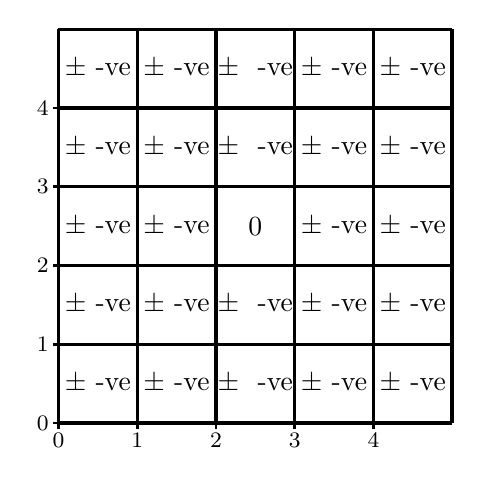
\begin{tikzpicture}
    % 1) Draw the bold 5×5 grid
    \draw[step=1cm, line width=1.2pt] (0,0) grid (5,5);

    % 2) Fill every cell except the center (i=2,j=2)
    \foreach \i in {0,...,4} {
      \foreach \j in {0,...,4} {
        % Skip the center cell (2,2)
        \ifnum\i=2\relax
          \ifnum\j=2\relax
            % do nothing here
          \else
            \node at (\i+0.5,\j+0.5) {$\pm$ \ -ve};
          \fi
        \else
          \node at (\i+0.5,\j+0.5) {$\pm$\ -ve};
        \fi
      }
    }

    % 3) Place the 0 in the very center
    \node at (2.5,2.5) {0};

    % 4) Add numeric ticks along the y-axis
    \foreach \y in {0,1,...,4} {
      \draw[line width=1pt] (0,\y) -- ++(-2pt,0);
      \node[left] at (0,\y) {\footnotesize \y};
    }

    % 5) Add numeric ticks along the x-axis
      \foreach \x in {0,1,...,4} {
        % Short tick mark
        \draw[line width=1pt] (\x,0) -- ++(0,-2pt);
        % Label just below
        \node[below] at (\x,0) {\footnotesize \x};
      }
\end{tikzpicture}
\end{center}

From our lemma we know that at least one of the cells in row 2 must be
negative and at least one of the cells in column 2 must be negative. The
2 negative numbers can go in positions $(2, a)$ and $(b, 2)$, where
$(i, j)$ denotes the cell in row $i$ and column $j$. We then must have
a negative number in column $a$ and one in row $b$. By simply placing a
negative number in cell $(b, a)$ we satisfy both those requirements in one
cell. All the other cells can be positive by construction, so in total we
have placed 3 negative numbers. All we need to
do to finish the problem is show that there exists a construction with
2 negative numbers in a row/column and 3 positive numbers where the middle
number is $x < 0$, since both row $b$ and column $a$ will have 2 negative
numbers. For some let the other 4 cells be $7x, -x, -x, -x$ in some order,
clearly all 5 numbers in the sequence are different since $x\neq 0$ and
$\frac{1}{5}(x+7x-x-x-x) = x$. This finishes the problem. $\blacksquare$
\end{solution}

\end{document}
